% Copyright (c)  2005-2010 EDF-EADS-PHIMECA.
% Permission is granted to copy, distribute and/or modify this document
% under the terms of the GNU Free Documentation License, Version 1.2
% or any later version published by the Free Software Foundation;
% with no Invariant Sections, no Front-Cover Texts, and no Back-Cover
% Texts.  A copy of the license is included in the section entitled "GNU
% Free Documentation License".
\renewcommand{\filename}{docUC_InputWithData_CloudDrawing.tex}
\renewcommand{\filetitle}{UC :  Drawing one cloud }

% \HeaderNNIILevel
% \HeaderIILevel
\HeaderIIILevel



\index{Graph!Clouds of points}
\index{View Image}
\index{Graph!Superposition of graphs}



The objective of this Use Case is to draw on a graph one point cloud of dimension 2.\\

Details on each object may be found in the User Manual  (\href{OpenTURNS_UserManual_TUI.pdf}{see User Manual - Graph / Cloud}).\\


\requirements{
  \begin{description}
  \item[$\bullet$] one numerical sample of dimension 2 : {\itshape sample}
  \item[type:]  NumericalSample
  \end{description}
}
{
  \begin{description}
  \item[$\bullet$] the files containing the cloud graph : {\itshape Graph\_Cloud\_OT.png, Graph\_Cloud\_OT.eps}
  \item[type:] files at format PNG or EPS or FIG
  \end{description}
}

\textspace\\
Python script for this UseCase :

\begin{lstlisting}
  # Create an empty graph
  myGraph = Graph("Sample", "x1", "x2", True, "topright")
  print  "myGraph=" , myGraph

  # Create the cloud Drawable
  # cloud : filled squares in blue
  myCloud = Cloud(sample, "blue", "fsquare","First Cloud")
  print  "myCloud=" , myCloud

  # Then, add it in the empty graph
  myGraph.addDrawable(myCloud1)

  # Impose a bounding box : x-range and y-range
  # boundingBox = [xmin, xmax, ymin, ymax]
  myBoundingBox = NumericalPoint( (xmin, xmax, ymin, ymax) )
  myGraph.setBoundingBox(myBoundingBox)

  # In order to see the graph without creating the associated files
  Show(myGraph)

  # Draw the graph containing the cloud
  myGraph.draw("Graph_Cloud_OT")

  # View the bitmap file
  ViewImage(myGraph.getBitmap())

  # Check if it worked
  print  "bitmap=" , myGraph.getBitmap()
  print  "postscript=" , myGraph.getPostscript()
\end{lstlisting}
\textspace\\



The following Figure (\ref{cloud2} draw the superposition of two clouds of dimension 2 and size 1000, realizations of
\begin{itemize}
\item a Normal distribution with $\vect{0}$ mean, unit standard deviation and independant components,
\item a Normal distribution with unit-mean,  unit-standard deviation and independant components.
\end{itemize}

\begin{figure}[H]
  \begin{center}
    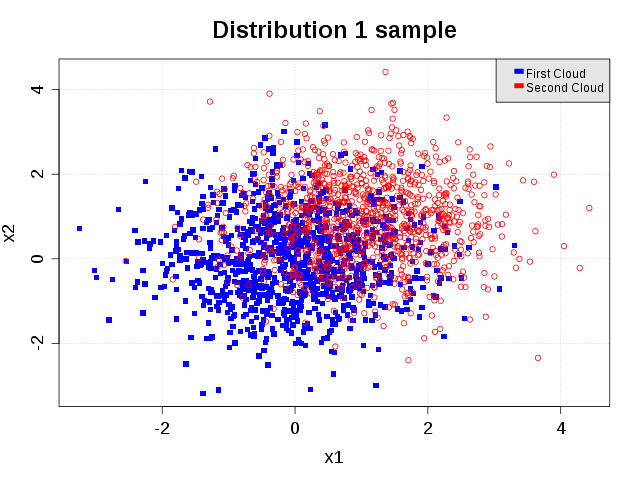
\includegraphics[width=10cm]{cloud2.png}
  \end{center}
  \caption{Superposition of two normal NumericalSample of dimension 2.}
  \label{cloud2}
\end{figure}

